\begin{figure*}[thp]
	\center
	\begin{subfigure}{0.7\textwidth}
		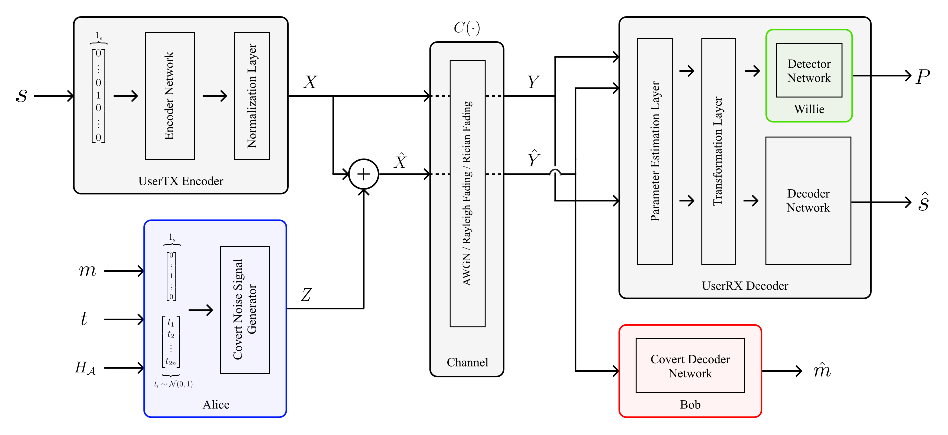
\includegraphics[width=\linewidth]{figs/system_architecture}
	\end{subfigure}
	\\
	\caption{Overall architecture of our system model in the single-user scenario. UserTX uses an encoder network to encode binary messages to a vector of signals and Alice transmits her covert signals into the shared channel. After passing through the channel, UserRX extracts the normal message, Bob decodes the covert message, and Willie tries to distinguish covert and normal signals from the signals. (Colored components are under the control of covert users and gray components are the non-controllable parts of the system)}	
	\label{fig:system_architecture}
\end{figure*}


\section{System Model}
\label{s:single-model}
In this section, we provide an overview of the system and define each actor's rule in our system model.

Our system consists of normal users who are communicating with each other via autonencoder wireless systems. This communication can either be single-user, i.e., communication between a single pair of a transmitter and a receiver, or multi-user, i.e., communication between multiple transmitters and a base station receiver. In the single-user setup, we referrer to the encoder or the transmitter as UserTX, and to the decoder or the receiver as UserRX. The multi-user system, on the other hand, has multiple transmitters (UserTXs) that are communicating with a single base station (BaseRX), which acts as a central receiver. These transmitters each uses their own encoder network to encode a binary message to a vector of signals. Their networks share no parameters and have no knowledge of other transmitters' messages. Each and every pair of UserTX and BaseRX forms an autoencoder model wherein UserTX represents the encoder and BaseRX accounts for the decoder network. In both single and multi-user systems, communication begins with UserTX encoding a binary message to a vector of signals using its encoder network. This vector of signals is then transmitted over the channel. We consider three channel models of AWGN, Rayleigh fading, and Rician fading. In the case of the multi-user system, as transmitters send their signals simultaneously over a shared channel, there will be interference at the receiver. In the end, a noisy version of the transmitted signal is received at the receiver side, where UserRX or BaseRX extracts the message(s) by decoding the signals. In the multi-user setup, BaseRX receives the signals from all transmitters using multiple antennas, and decodes the messages in the same way UserRX does. The only difference is that BaseRX handles the decoding process not just for one but for all the transmitters' signals in one pass. In the case of fading channels, before the receiver pass the signals to the decoder network, it equalizes them using the channel matrix. This channel matrix is estimated by the receiver in the single-user system and is provided to the decoder in the multi-user system. Figures \ref{fig:system_architecture}, and \ref{fig:multi_system_architecture} show an overview of our system model in both single-user and multi-user scenarios.

On the other hand, we have the covert user whose objective is to establish a hidden communication in the above system without arousing the observer's suspicions. There is a covert sender (Alice) who wants to secretly communicate with her intended receiver (Bob). Bob's is an adversary access point and his existence is no secret to the other entities of the system. However, if anyone tries to secretly communicate with him, system's observer (Willie) will mitigate their communication and shut it down. Willie listens to all the ongoing transmissions on the channel and uses a binary classifier network that tells how probable it is for each signal to be covert or normal. Any distortion in the normal signals can be a sign for Willie that there is a covert trasnmission, and thereby Alice has to pick her covert signals carefully. That means, she should not make any noticeable changes to the statistical properties of the channel noise or the other normal signals. On the other hand, covert signals should not  amplify the error rate of the system, because an unexpected increase in the error rate can also raise suspicion. We consider Willie to be an integrated module at the receiver of the normal communication system, i.e., UserRX in the single-user and BaseRX in the multi-user system. This way not only can he detect the incoming covert signals, but also measure the communication's error rate. We represent all these three roles by DNNs that are put in a training setup similar to the GANs. An adversarial training setting as such ensures that the optimal solution is only achieved when they all reach an equilibrium at the end of the training.

The covert communication starts with Alice using her generative model to embed a confidential message into a covert noise vector. In the case of non-fading channels, Alice merely needs a covert message and a random trigger to produce a covert signal. However, in fading channels, she needs the channel state information of her channel to Bob in the single-user system, and also other users to Bob in the multi-user system. This information can be provided to Alice by Bob, who can listen to the broadcasted pilot signals of other transmitters and measure the channel state. Since there is no necessity for Bob to hide his existence, he can freely broadcast this information as an access point. Next, Alice produces the signals and transmits them into the shared channel regardless of what other users' transmissions are. That means, her covert signals should be agnostic to the normal signals. After getting mixed with other users' transmissions and distorted by the channel effects, Bob receives this signal and extracts Alice's message from it. Unlike the receiver or the observer, here we assume Bob to only have one antenna at his receiver. To keep their communication hidden from Willie, Alice and Bob incorporates a statistical undetectability constraint on the produced covert signals by optimizing their transmissions against his network. When Willie's classifier can do almost no better than random guessing in detecting covert and normal signals, we can safely assume a low probability of detection covert communication is achieved.


\begin{figure*}[thp]
	\center
	\begin{subfigure}{0.7\textwidth}
		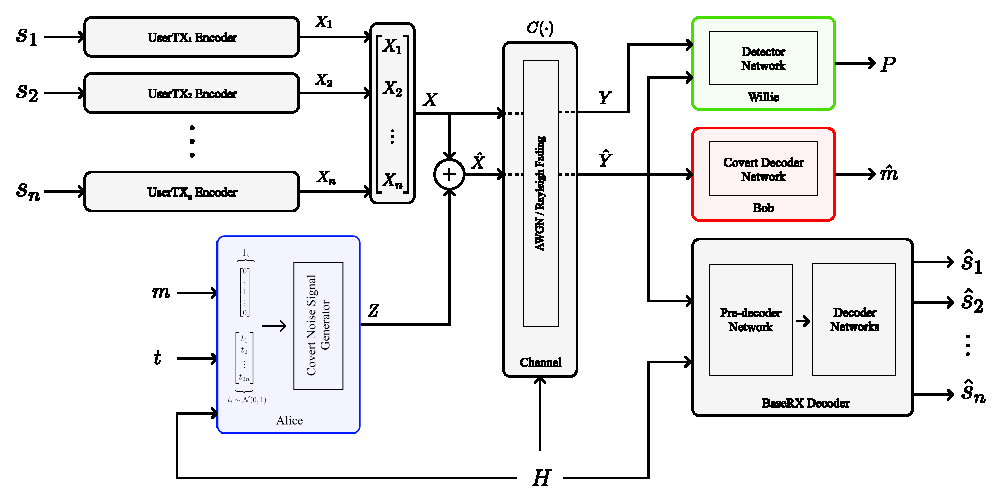
\includegraphics[width=\linewidth]{figs/multi_system_architecture}
	\end{subfigure}
	\\
	\caption{Overall architecture of our system model in the single-user scenario. Each UserTX uses its own encoder network to encode binary messages to a vector of signals and Alice transmits her covert signals into the shared channel. After passing through the channel, BaseRX extracts the normal messages, Bob decodes the covert message, and Willie tries to distinguish covert and normal signals from the signals. (Colored components are under the control of covert users and gray components are the non-controllable parts of the system)}
	\label{fig:multi_system_architecture}
\end{figure*}

\section{GAN-Based Covert Model}
For a given binary secret message \(m\), Alice first one-hot encodes the message and then uses its generator model to produce a covert noise signal \(Z\). Having such a stochastic generative model for Alice results in each covert message getting mapped to a set of different covert noise signals instead of one. She then transmits this covert signal to the shared channel between all entities of the system. This covert signal mixes with the other transmitters' signals \(X\) and forms the mixed covert signal \(\hat{X}\). 

\begin{equation}
	\hat{X} = X + Z.
\end{equation}

As we mentioned before, we consider three channel models of AWGN, Rayleigh fading, and Rician fading. Therefore, there will be three different channel outputs for these three channel models. We use a mapping function \(\mathcal{C}(\cdot)\) to express each of these channels' outputs. Since signals in the multi-user system also experience interference, we express single-user and multi-user channel's outputs separately.

\textit{AWGN Channel Output}: For the AWGN channel model, the signal received at the receiver carries within itself the channel's noise effect \(N \sim \mathcal{N}(0, \sigma^2)\). Consequently, the channel function \(\mathcal{C}(\cdot)\) and the final covert signal \(\hat{Y}\) in the single-use system can be represented as:
\begin{equation}
	\hat{Y} = \mathcal{C}(\hat{X}) = X + Z + N.
\end{equation}
For the multi-user system, signals also get distorted by the channel interference effect. This is due to the multiple transmitters sending their signals at the same time. Consequently, the resulting covert signal can be denoted as:
\begin{equation}
	 \hat{Y} = \mathcal{C}(\hat{X}) = \sum^{i \in U}X_i + Z + N.
\end{equation}
where \(U\) is the set that contains all transmitters.

\textit{Rayleigh and Rician Fading Channel Outputs}: For the Rayleigh and Rician fading channel models, we consider a flat-frequency block-fading channel where each vector of signals, which corresponds to a codeword, is assumed to be faded independently. Let \(H_{\mathcal{U}}\) be the fading coefficient for the signal vector \(X\), and \(H_{\mathcal{A}}\) be the fading coefficient for Alice's signal, then the channel function \(\mathcal{C}(\cdot)\) and the final covert signal \(\hat{Y}\) in the single-user system is given by:
\begin{equation}
	\hat{Y} = \mathcal{C}(\hat{X}) = (H_{\mathcal{U}} \cdot X) + (H_{\mathcal{A}} \cdot Z) + N.
\end{equation}

In the multi-user case, the final covert signal including the channel interference can be written as:
\begin{equation}
	\hat{Y} = \mathcal{C}(\hat{X}) = \sum^{i \in U}(H_{\mathcal{U}_i} \cdot X_i) + (H_{\mathcal{A}} \cdot Z) + N.
\end{equation}

On the receiver side, Bob receives this distorted covert signal \(\hat{Y}\) and uses his decoder network to reconstruct the covert message \(\hat{m}\).

The statistical properties of signals transmitted over the channel are captured by the Willie's network. This network's objective is to classify sequences of normal \(Y\) and covert signals \(\hat{Y}\) and provide useful feedback to Alice during training. This feedback helps Alice modify the produced covert signals such that they are indistinguishable from the normal transmitted signals. This ensures that when model is deployed in a real communication setup, it is highly unlikely for the system's observer to detect the covert transmissions.

\subsection{General Formulation}
\textbf{Reliability}: The very first objective of our covert model is to have a working covert communication. To this end, Bob has to have a plausible accuracy in decoding covert messages that Alice sends through the covert signals \(\hat{Y}\). As mentioned earlier, Alice employs a generative model that generates covert noise signals that correspond to the covert messages. Let \(\Theta_{\mathcal{A}}(\cdot)\) be the underlying function of Alice's generative model that takes a random trigger \(t \sim \mathcal{N}(0, 1)\), a covert message \(m\), the channel coefficients from Alice to Bob \(H_{\mathcal{A}}\), and in the multi-user system, the channel matrix \(H_{\mathcal{U}}\) and produces a covert signal \(Z\). The corresponding covert signal then can be denoted as \(Z_{m, t} = \Theta_{\mathcal{A}}(m, t, H_{\mathcal{A}}\footnotemark[1]), H_{\mathcal{U}}\footnotemark[2])\)). Let also  \(\Theta_{\mathcal{B}}(\cdot)\) be the underlying function of the decoder network that Bob utilizes to reconstruct the covert message \(\hat{m}\). Then the reliability of communication between Alice and Bob is achieved using the below loss function:
\begin{equation}
	\begin{aligned} \label{bob_loss}
	\mathcal{L}_{\mathcal{B}} & = \mathbb{E}_{m}[\mathcal{H}(\hat{m}, m)] \\
	& = \mathbb{E}_{m}[\mathcal{H}(\Theta_{\mathcal{B}}(\hat{Y}), m)] \\ 
	& = \mathbb{E}_{m}[\mathcal{H}(\Theta_{\mathcal{B}}(\mathcal{C}(\hat{X}), m)] \\ 
	& = \mathbb{E}_{m}[\mathcal{H}(\Theta_{\mathcal{B}}(\mathcal{C}(\Theta_{\mathcal{A}}(m, t, H_{\mathcal{A}}) + X)), m)].
	\end{aligned}
\end{equation}

For the multi-user system, this equation is written as:
\begin{equation}
	\begin{aligned}
		\mathcal{L}_{\mathcal{B}} & = \mathbb{E}_{m}[\mathcal{H}(\hat{m}, m)] \\
		& = \mathbb{E}_{m}[\mathcal{H}(\Theta_{\mathcal{B}}(\mathcal{C}(\Theta_{\mathcal{A}}(m, t, H_{\mathcal{A}}, H_{\mathcal{U}}) + X)), m)].
	\end{aligned}
\end{equation}
where \(\mathcal{H}(\cdot)\) is the cross entropy between the probability of reconstructed covert message \(\hat{m}\) and the actual covert message \(m\). This equation can be used to optimize both Alice's and Bob's networks by freezing one or the other's network parameters iteratively. 

\footnotetext[1]{This is an extra input parameter that is only used in systems with fading channel.}
\footnotetext[2]{This is an extra input parameter that is only used in the multi-user system with fading channel.}

\textbf{Low Interference}: While (\ref{bob_loss}) ensures the communication accuracy, we also need to verify that the generated perturbations leave no detrimental impact on the normal communication between UserTX and UserRX, otherwise, this can alert Willie of an abnormal activity taking place. To this end, we add a constraint that minimizes the UserRX's loss function during Alice's training. In the single-user system, we express it as:
\begin{equation}
	\begin{aligned} \label{alice_user_loss}
	\mathcal{L}_{\mathcal{U}} & = \mathbb{E}_{m}[\mathcal{H}(\hat{s}, s)] \\
	& = \mathbb{E}_{m}[\mathcal{H}(\Theta_{\mathcal{U}}(\hat{Y}), s)] \\
	& = \mathbb{E}_{m}[\mathcal{H}(\Theta_{\mathcal{U}}(\mathcal{C}(Z + X)), s)] \\
	& = \mathbb{E}_{m}[\mathcal{H}(\Theta_{\mathcal{U}}(\mathcal{C}(\Theta_{\mathcal{A}}(m, t, H_{\mathcal{A}}) + X)), s)].
	\end{aligned}
\end{equation}
where \(\Theta_{\mathcal{U}}(\cdot)\) is UserRX's decoder network function. Note that UserRX's decoder network is frozen during this training and only Alice's parameters will get updated.

For the multi-user system, since we have multiple transmitters sending signals, we need to minimize the BaseRX's loss function over all individual transmitters' signals. Thus, equation \ref{alice_user_loss} is rewritten as:
\begin{equation}
	\begin{aligned} \label{multi_alice_user_loss}
		\mathcal{L}_{\mathcal{U}} & = \sum^{i \in U}\mathbb{E}_{m}[\mathcal{H}(\hat{s}_i, s_i)] \\
		= \sum^{i \in U} & 
			\mathbb{E}_{m}[\mathcal{H}
			((\Theta_{\mathcal{U}}(\mathcal{C}(\Theta_{\mathcal{A}}(m, t, H_{\mathcal{A}}, H_{\mathcal{U}}) + X_i),  H_{\mathcal{U}}), s_i)].
	\end{aligned}
\end{equation}

\begin{algorithm}[tp!]
	\caption{Optimizing covert models algorithm}\label{alg:cap}
	\small
	\begin{algorithmic}
		\State $X \gets$ normal signals data
		\State $S, M \gets$ normal and covert messages sets
		\State $\Theta_{\mathcal{A}}, \Theta_{\mathcal{B}}, \Theta_{\mathcal{W}} \gets$ Alice, Bob, and Willie network functions
		\State $\Theta_{\mathcal{U}} \gets$ UserRX decoder network function
		\State $\mathcal{H} \gets$ cross entropy function
		\State $\mathcal{C} \gets$ channel mapping function
		\For{epoch $ep \in \{1 \ldots n_{epochs}$\}}
		\State $t \sim \mathcal{N}(0, 1)$
		\State $\mathcal{L}_{\mathcal{W}} = \mathcal{H}(\mathcal{C}(X), \mathcal{C}(\Theta_{\mathcal{A}}(M, t, H_{\mathcal{A}}, H_{\mathcal{U}}) + X))$
		\State Update $\Theta_{\mathcal{W}}$ to minimize $\mathcal{L}_{\mathcal{W}}$
		\State $\mathcal{L}_{\mathcal{B}} = \mathcal{H}(\mathcal{C}(\Theta_{\mathcal{A}}(M, t, H_{\mathcal{A}}, H_{\mathcal{U}}) + X), M)$
		\State Update $\Theta_{\mathcal{B}}$ to minimize $\mathcal{L}_{\mathcal{B}}$
		\State $\mathcal{L}_{\mathcal{U}} \gets \mathcal{H}(\Theta_{\mathcal{U}}(\mathcal{C}(\Theta_{\mathcal{A}}(M, t, H_{\mathcal{A}}, H_{\mathcal{U}}) + X)), S)$
		\State
		$\mathcal{L}_{\mathcal{A}} = \lambda_{\mathcal{B}} \mathcal{L}_{\mathcal{B}} + \lambda_{\mathcal{U}} \mathcal{L}_{\mathcal{U}} - \lambda_{\mathcal{W}} \mathcal{L}_{\mathcal{W}}$
		\State Update $\Theta_{\mathcal{A}}$ to minimize $\mathcal{L}_{\mathcal{A}}$
		\EndFor
	\end{algorithmic}
\end{algorithm}

\textbf{Undetectability}: In our model, Willie acts as a critic network, similar to what is known as a discriminator in GAN models \cite{goodfellow2014generative}. The so-called real and fake samples in GANs' discriminator training process here are mapped to normal and covert signals, respectively. That is, for the single-user system we use the below loss function to optimize Willie's network to classify covert and normal signals:
\begin{equation}
	\begin{aligned} \label{willie_loss}
	\mathcal{L}_{\mathcal{W}} & = \mathbb{E}_{m}[\mathcal{H}(\hat{y}, y)] \\
	& = \mathbb{E}_{m}[\mathcal{H}(\mathcal{C}(\hat{X}), \mathcal{C}(X))] \\
	& = \mathbb{E}_{m}[\mathcal{H}(\mathcal{C}(\Theta_{\mathcal{A}}(m, t, H_{\mathcal{A}}) + X), \mathcal{C}(X))].
	\end{aligned}
\end{equation}
where \(\mathcal{H}(\cdot)\) is the binary cross entropy between the covert signals \(\hat{Y}\) and the normal signals \(Y\). 

And again for the multi-user system, we need to optimize the Willie's network over all the transmitters' outputs.

\begin{equation}
	\begin{aligned} \label{multi_willie_loss}
		\mathcal{L}_{\mathcal{W}} & = 
		\sum^{i \in U} \mathbb{E}_{m}[H(\hat{Y}, Y)] \\
		& = \sum^{i \in U}
			\mathbb{E}_{m}[\mathcal{H}(\mathcal{C}(\Theta_{\mathcal{A}}(m, t, H_{\mathcal{A}}, H_{\mathcal{U}}) + X), \mathcal{C}(X))].
	\end{aligned}
\end{equation}

This white-box adversarial training against Alice's network ensures that the Willie's network will be adequately trained to tell covert and normal signals apart. On the other hand, we do not want the covert signals that Alice produces to deviate from the statistical properties of the normal signals on the channel, otherwise it is likely that the observer of the channel detects and mitigates the covert communication. To achieve this undetectability property, we utilize Willie's network to play the role of a discriminator network in Alice's optimization function. In other words, Alice training against this network results in maximizing Willie's uncertainty about his predictions and having a regularizer as such helps Alice and Bob to form their covert communication in a way that is indistinguishable from the actual channel's noise, yet understandable by both. Altogether, Alice's loss function can be expressed as a weighted sum of these three objectives:
\begin{equation}
	\begin{array}{l} \label{alice_loss}
	\mathcal{L}_{\mathcal{A}} = \lambda_{\mathcal{B}} \mathcal{L}_{\mathcal{B}} + \lambda_{\mathcal{U}} \mathcal{L}_{\mathcal{U}} - \lambda_{\mathcal{W}} \mathcal{L}_{\mathcal{W}}.
\end{array}
\end{equation}
where \(\lambda_{\mathcal{B}}\), \(\lambda_{\mathcal{U}}\), and \(\lambda_{\mathcal{W}}\) determine the importance of Alice's objectives. Algorithm \ref{alg:cap} summarizes the procedure by which we train our covert models.

\begin{figure*}[!tp]
	\center
	\begin{subfigure}{0.28\textwidth}
		\includegraphics[width=\linewidth]{figs/autoencoder_bler_awgn}
		\caption{AWGN channel}
	\end{subfigure}
	\begin{subfigure}{0.28\textwidth}
	\includegraphics[width=\linewidth]{figs/autoencoder_bler_rician}
	\caption{Rician fading channel}	
	\end{subfigure}
	\begin{subfigure}{0.28\textwidth}
		\includegraphics[width=\linewidth]{figs/autoencoder_bler_rayleigh}
		\caption{Rayleigh fading channel}	
	\end{subfigure}
	\caption{Autoencoders performance in terms of BLER over a range of SNR values in our single-user system. Models are trained over AWGN, Rayleigh and Rician fading channels for a set of parameters that has the same data rate.}
	\label{fig:autoencoder_bler}
\end{figure*}

\subsection{Neural Network Architecture}
\textbf{User's Autoencoder Network}: Autoencoder model accepts a binary message \(s\) of size \(k\) bits and outputs a reconstructed version of it \(\hat{s}\). The encoder maps the message to a vector of signals of size \(2 \times n\), where \(n\) is the number of channel uses, through one-hot encoding. Since there are multiple encoders in the multi-user system, the resultant vector will be of size \(n_{tx} \time 2 \times (2 \times n)\). The signals generated from the encoder are then passed to the channel mapping function that incorporates the channel noise and interference effects. When the channel model has fading and the system is single-user, the receiver side utilizes the two layers of parameter estimation and transformation to equalize the signals. We apply a simple transformation function that divides signals by the channel fading coefficients estimated via the parameter estimation layer. Note that more complex transformation functions can be used and are described in \cite{o2017introduction}, however optimizing the performance of the autoencoder model is out of the scope of this article. In the multi-user system, channel coefficients are given as an input to the decoder. Therefore, BaseRX equalizes the received signals using zero-forcing technique \cite{garg2010wireless}. In the single-user system, UserRX eventually reconstructs the message using its decoder network. In the multi-user system, BaseRX receives signals from all the transmitters at once and decodes them simultaneously by first passing the signals to a pre-decoder network and then using separate decoders at the ending layers.


\textbf{Alice's Network}: Alice first transforms a covert message \(m\) to its corresponding one-hot encoding representation so that each message belongs to a unique class. Then she uses a random trigger \(t\), which is to randomize the process by which the covert noise signal \(Z\) is produced, along with the channel coefficients \(H_{\mathcal{A}}\) and \(H_{\mathcal{U}}\). For Alice's generator model, we use multiple dense layers with ReLU and Tanh activation functions. The first layer of this model takes in the inputs and acts as an embedding layer by enlarging the input's domain space. The following fully connected layers are to extract the useful features and do the encoding process. The last layer of this model does a dimension transformation so that the generated covert signal \(Z\) complies with the dimension of the normal signal \(X\) on the channel. 


\textbf{Bob's Network}: Bob receives this covert signal \(\hat{Y}\) that has undergone the channel's effects and feeds it through its decoder network to extract the secret message. We use a more sophisticated network for him compared to Alice since decoding such a distorted signal is a much more complex task. The received message by Bob first goes through the first layer of the network, which is a wide dense layer followed by a Tanh activation function, to increase the input's feature space. Then the data is passed through multiple 1-Dimensional Convolutional (1D Conv) layers that learn the coding that Alice has developed to encode the covert messages. We find that using 1D Conv layers helps Bob and Alice achieving a better consistency in the accuracy of their communication, especially when the channel model is more complicated (i.e., when there is also fading in the channel). The rest of Bob's decoder network consists of two dense layers that do a domain remapping from the learned feature space to the covert message domain space. Similar to UserRX's and BaseRX's decoder networks, Bob eventually predicts the covert message by doing a classification on the received signal.


\textbf{Willie's Network}: Willie receives both the covert signal \(\hat{Y}\) and the normal signal \(Y\) and outputs a confidence probability \(P\) on how probable it is for the signal to be normal. We choose the same network architecture as Bob's for Willie except for the last layer that has a Sigmoid activation function instead of Softmax. Using the same network for both ensures Bob and Willie will have the same capacity for training and can compete each other in a fair setup.